\chapter{\label{ch:ch4} Design ad Implementation}

This chapter outlines the design and implementation phases of the mobile robot system project. The purpose of this chapter is to describe the system’s architecture, the design of each subsystem, the integration of hardware and software, and how these components work together to achieve the goals of this project. The design emphasizes ease of navigation, real-time feedback, and effective control via an intuitive interface.

\section{\label{sec:ch4_firstsec}System Design}

The design of the mobile robot system was based on the specific project requirements outlined in Chapter\ref{ch:req_and_specs}. Following a detailed review of relevant literature and an analysis of system needs, the robot’s overall design was established. The architecture integrates several key components—Raspberry Pi, camera module, fiducial markers, motor control system, and wireless communication modules—to ensure optimal system performance.

The core decision-making process involved selecting the appropriate technologies and components. Based on the findings from previous research (e.g., Jacobsen et al. \cite{jacobsen2018}, La Delfa et al. \cite{delfa2015}, and Vanitha et al. \cite{vanitha2016}), which explored various mobile robot control methods using augmented reality (AR) and computer vision, it became clear that a Raspberry Pi-based system with a web interface would provide the required flexibility and ease of control for this project.

After evaluating several options for actuation and navigation, it was determined that motorized control through a motor driver and a four-wheel drive system would provide the most reliable and efficient solution for movement. This decision was supported by studies that demonstrate the performance of motor-driven robots in both laboratory and dynamic environments. Additionally, the use of fiducial markers, such as ArUco or AprilTag markers, was identified as a robust solution for localization and obstacle avoidance (La Delfa et al. \cite{delfa2015}; Vanitha et al. \cite{vanitha2016}).

The integration of these components into a cohesive design was a critical aspect of the project. The Raspberry Pi was chosen as the central processing unit because of its ability to handle computer vision tasks and interface with the hardware seamlessly. The camera module was selected to provide real-time video streaming, which not only serves as an input for the robot’s environment perception but also allows for remote monitoring through the web interface.

\begin{figure}[H]
	\centering
	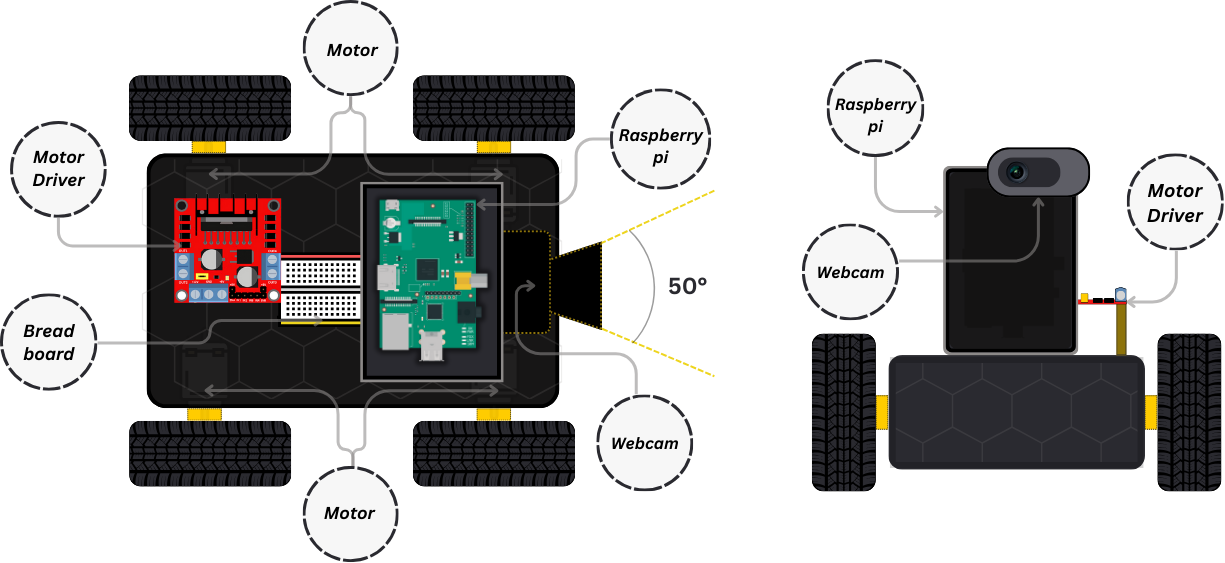
\includegraphics[width=1\textwidth]{ch4/figs/robot_car.png}
	\caption{Illustration of the hardware layout, showing the arrangement of key components like the Raspberry Pi, motor system, and camera module.}
	\label{fig:hardware_layout}
\end{figure}


\section{\label{sec:sys_architecture} System Architecture}

The project is composed of several key components, below is a high level overview of all the components that are needed in order execute the project properly.

\begin{table}[ht]
\centering
\caption{System Architecture Components}
\label{tab:system_architecture}
\begin{tabular}{|p{5cm}|p{10cm}|}
\hline
\textbf{Component} & \textbf{Description} \\ \hline
Microcontroller/Processor & Manages computer vision algorithms and interfaces with hardware. Responsible for overall system control and data processing. \\ \hline
Web Camera & Provides real-time video feed for remote monitoring and vision tasks. Captures high-quality images for processing. \\ \hline
Motor and Drive System & Four-wheel drive system for robot mobility. Includes motors and a motor controller for precise movement control.\\ \hline
Fiducial Markers & Visual markers (e.g., ArUco or AprilTag) placed in the environment to assist with localization and navigation.\\ \hline
Web-based Control Interface & Allows remote control of the robot’s movements and camera functions, with video streaming capabilities. \\ \hline
Power Supply & Provides electrical power to all components of the system. Needs to support extended operation and peak power demands. \\ \hline
Chassis & Physical structure of the robot that houses and protects all components. Designed for durability and optimal component placement.  \\ \hline
Sensors & Additional sensors for environmental awareness (e.g., ultrasonic sensors, IMU, GPS).\\  \hline
Communication Module & Enables wireless communication between the robot and the control interface, supporting long-range and reliable data transmission. \\ \hline
\end{tabular}
\end{table}
